% !TEX encoding = UTF-8
% !TEX TS-program = pdflatex
% !TEX root = ../tesi.tex
\subsection{UC5 - Elaborazione metadati}
\begin{itemize}
  \item \textbf{Identificativo}: UC5
  \item \textbf{Nome}: elaborazione metadati
  \item \textbf{Descrizione grafica}:
\end{itemize}

\begin{figure}[H]
  \centering
  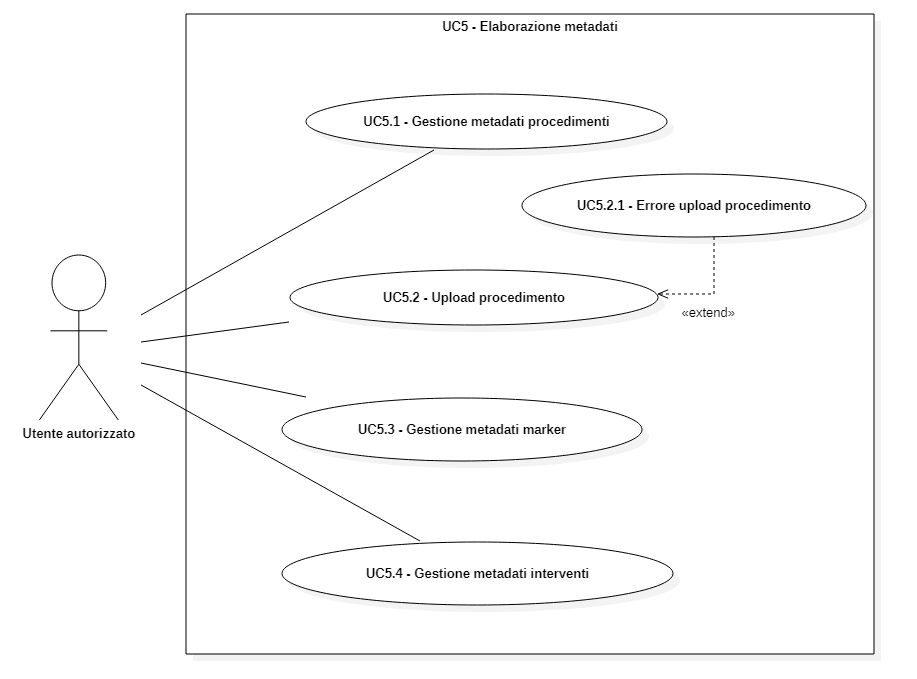
\includegraphics[width=\textwidth]{immagini/usecase/UC5.png}
  \caption{Descrizione grafica caso d'uso UC5}
\end{figure}

\begin{itemize}
  \item \textbf{Attori}
        \begin{itemize}
          \item \textit{Primari}: utente autorizzato
        \end{itemize}
  \item \textbf{Precondizione}: l'utente si trova sulla pagina di visualizzazione dei file con i relativi metadati.
  \item \textbf{Postcondizione}: l'utente ha visualizzato ed eventualmente elaborato i metadati desiderati.
  \item \textbf{Scenario principale}: l'utente può visualizzare i metadati relativi ad ogni file caricato.
  \item \textbf{Scenario secondario}: l'utente può gestire (modificare aggiungere eliminare) i procedimenti relativi ad ogni file. (\textbf{UC5.1})
  \item \textbf{Scenario secondario}: l'utente può gestire (modificare aggiungere eliminare) i marker relativi ad ogni file. (\textbf{UC5.3})
  \item \textbf{Scenario secondario}: l'utente può gestire (modificare aggiungere eliminare) gli interventi relativi ad ogni file. (\textbf{UC5.4})
\end{itemize}

% \subsubsection{UC5.1 - Visualizzazione metadati}
% \begin{itemize}
%   \item \textbf{Identificativo}: UC5.1
%   \item \textbf{Nome}: visualizzazione metadati
%   \item \textbf{Descrizione grafica}: (approfondita in UC5)
%   \item \textbf{Attori}
%         \begin{itemize}
%           \item \textit{Primari}: utente autorizzato
%         \end{itemize}
%   \item \textbf{Precondizione}: l'utente vuole visualizzare i metadati relativi ad un file.
%   \item \textbf{Postcondizione}: l'utente visualizza i metadati del file.
%   \item \textbf{Scenario principale}: l'utente visualizza i metadati relativi al file come Marker, Interventi e Procedimenti.
%   \item \textbf{Scenario secondario}: l'utente può elaborare i metadati del file. (\textbf{UC5.2}, \textbf{UC5.4}, \textbf{UC5.5})
% \end{itemize}

\subsubsection{UC5.1 - Gestione metadati Procedimenti}
\begin{itemize}
  \item \textbf{Identificativo}: UC5.1
  \item \textbf{Nome}: getione metadati Procedimenti
  \item \textbf{Descrizione grafica}: (approfondita in UC5)
  \item \textbf{Attori}
        \begin{itemize}
          \item \textit{Primari}: utente autorizzato
        \end{itemize}
  \item \textbf{Precondizione}: l'utente vuole elaborare procedimenti relativi ad un file.
  \item \textbf{Postcondizione}: l'utente ha elaborato i procedimenti.
  \item \textbf{Scenario principale}: l'utente può modificare, aggiungere o eliminare i procedimenti relativi ad un file.
\end{itemize}

\subsubsection{UC5.2 - Upload procedimento}
\begin{itemize}
  \item \textbf{Identificativo}: UC5.2
  \item \textbf{Nome}: upload procedimento
  \item \textbf{Descrizione grafica}: (approfondita in UC5)
  \item \textbf{Attori}
        \begin{itemize}
          \item \textit{Primari}: utente autorizzato
        \end{itemize}
  \item \textbf{Precondizione}: l'utente vuole fare l'upload dei metadati riguardanti un procedimento relativi ad un file.
  \item \textbf{Postcondizione}: l'utente ha fatto l'upload del procedimento desiderato.
  \item \textbf{Scenario principale}: l'utente può tramite un apposito bottone fare l'upload del file e i relativi metadati del procedimento che desidera.
  \item \textbf{Scenario secondario}: si è verificato un errore nella richiesta di upload del procedimento. (\textbf{UC5.2.1})
\end{itemize}

\subsubsection{UC5.2.1 - Errore upload procedimento}
\begin{itemize}
  \item \textbf{Identificativo}: UC5.2.1
  \item \textbf{Nome}: errore upload procedimento
  \item \textbf{Descrizione grafica}: (approfondita in UC5)
  \item \textbf{Attori}
        \begin{itemize}
          \item \textit{Primari}: utente autorizzato
        \end{itemize}
  \item \textbf{Precondizione}: il sistema non ha gestito correttamente la richiesta di upload procedimento.
  \item \textbf{Postcondizione}: l'errore viene visualizzato sull'applicazione.
  \item \textbf{Scenario principale}: la richiesta di upload procedimento non va a buon fine e l'errore viene mostrato all'utente.
\end{itemize}


\subsubsection{UC5.3 - Gestione metadati Marker}
\begin{itemize}
  \item \textbf{Identificativo}: UC5.3
  \item \textbf{Nome}: getione metadati Marker
  \item \textbf{Descrizione grafica}: (approfondita in UC5)
  \item \textbf{Attori}
        \begin{itemize}
          \item \textit{Primari}: utente autorizzato
        \end{itemize}
  \item \textbf{Precondizione}: l'utente vuole elaborare i marker relativi ad un file.
  \item \textbf{Postcondizione}: l'utente ha elaborato i marker.
  \item \textbf{Scenario principale}: l'utente può modificare, aggiungere o eliminare i marker relativi ad un file.
\end{itemize}

\subsubsection{UC5.4 - Gestione metadati Interventi}
\begin{itemize}
  \item \textbf{Identificativo}: UC5.4
  \item \textbf{Nome}: getione metadati Intervetni
  \item \textbf{Descrizione grafica}: (approfondita in UC5)
  \item \textbf{Attori}
        \begin{itemize}
          \item \textit{Primari}: utente autorizzato
        \end{itemize}
  \item \textbf{Precondizione}: l'utente vuole elaborare gli interventi relativi ad un file.
  \item \textbf{Postcondizione}: l'utente ha elaborato gli interventi.
  \item \textbf{Scenario principale}: l'utente può modificare, aggiungere o eliminare gli interventi relativi ad un file.
\end{itemize}
\newpage